\documentclass[12pt]{article} 
\usepackage[utf8]{inputenc}
\usepackage{geometry}
\geometry{letterpaper}
\usepackage{graphicx} 
\usepackage{parskip}
\usepackage{booktabs}
\usepackage{array} 
\usepackage{paralist} 
\usepackage{verbatim}
\usepackage{subfig}
\usepackage{fancyhdr}
\usepackage{sectsty}

\pagestyle{fancy}
\renewcommand{\headrulewidth}{0pt} 
\lhead{}\chead{}\rhead{}
\lfoot{}\cfoot{\thepage}\rfoot{}

%%% SECTION TITLE APPEARANCE
\allsectionsfont{\sffamily\mdseries\upshape} 

%%% ToC (table of contents) APPEARANCE
\usepackage[nottoc,notlof,notlot]{tocbibind} 
\usepackage[titles,subfigure]{tocloft}
\renewcommand{\cftsecfont}{\rmfamily\mdseries\upshape}
\renewcommand{\cftsecpagefont}{\rmfamily\mdseries\upshape} %

\usepackage{amsmath}
\usepackage{amssymb}

\title{APMA 0350: Homework 6}
\author{Milan Capoor}
\date{11 October 2022}

\begin{document}
\maketitle

\textbf{Problem 1: Solve the system and draw a phase portrait}
\[x' = \begin{bmatrix}
    -1 & -4\\
    1 & -1
\end{bmatrix}x\]

Eigenvalues:
\[\begin{vmatrix}
    -1 & -4\\
    1 & -1
\end{vmatrix} = (-1 - \lambda)^2 + 4 = \lambda^2 + 2 \lambda + 5 = 0\]
\[\lambda = \frac{-2 \pm \sqrt{4- 4(5)}}{2} = -1 \pm 2i\]

Eigenvector $\lambda = -1 + 2i$:
\[\begin{array}{c c | c}
    -2i & -4 & 0\\
    1 & -2i    
\end{array} \sim \begin{array}{c c | c}
    -2i & -4 & 0\\
    0 & 0 & 0
\end{array}\]
\[\implies -2ix_1 - 4x_2 = 0\]
\[\vec{v}_{\lambda = -1 + 2i} = \begin{bmatrix}
    2\\
    -i
\end{bmatrix}\]

Solution:
\[e^{(-1 + 2i)t} \begin{bmatrix}
    2 + 0i\\
    0 - i
\end{bmatrix} = e^{-t}\; e^{2it} \left(\begin{bmatrix}
    2\\0
\end{bmatrix} + i\begin{bmatrix}
    0\\
    -1
\end{bmatrix}\right)\]
\[= e^{-t}\left(\cos 2t + i \sin 2t\right) \left(\begin{bmatrix}
    2\\0
\end{bmatrix} + i\begin{bmatrix}
    0\\
    -1
\end{bmatrix}\right)\]

\[\boxed{\vec{x}(t) = C_1 e^{-t} \left(\cos 2t \begin{bmatrix}
    2\\0
\end{bmatrix} - \sin 2t \begin{bmatrix}
    0\\-1
\end{bmatrix}\right) + C_2 e^{-t} \left(\cos 2t \begin{bmatrix}
    0\\-1
\end{bmatrix} + \sin 2t \begin{bmatrix}
    2\\0
\end{bmatrix}\right)}\]

Phase portrait:

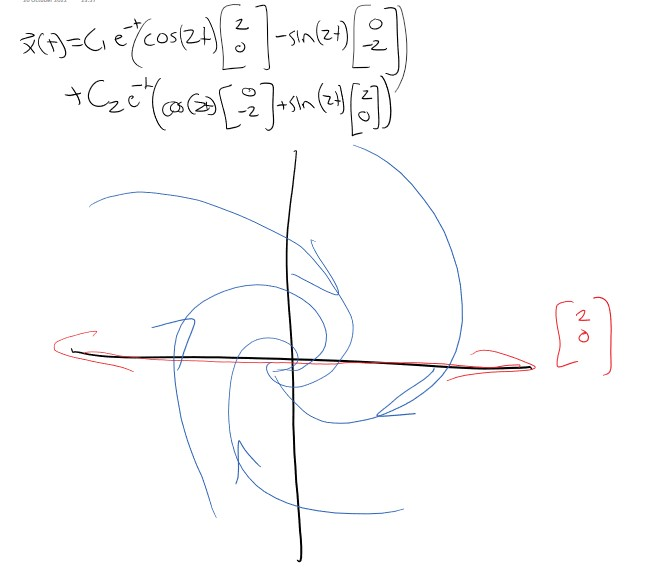
\includegraphics{Images/phase.jpg}

\pagebreak

\textbf{Problem 2:} Solve the following system
\begin{enumerate}
    \item 
    \[x' = \begin{bmatrix}
        -3 & 2\\
        -1 & -1
    \end{bmatrix}x, \quad x(0) = \begin{bmatrix}
        1\\-2
    \end{bmatrix}\]

    Eigenvalues:
    \[\begin{vmatrix}
        -3 & 2\\
        -1 & -1
    \end{vmatrix} = (-2 - \lambda)(-1 - \lambda) + 2 = \lambda^2 + 4\lambda + 5 = 0\]
    \[\lambda = \frac{-4 \pm \sqrt{16 - 4(5)}}{2} = -2 \pm i\]

    Eigenvector for $\lambda = -2 - i$:
   \[ \begin{array}{c c | c}
        -1 + i & 2 & 0\\
        -1 & 1 + i & 0
    \end{array} \sim \begin{array}{c c | c}
        -1 + i & 2 & 0\\
        0 & 0 & 0
    \end{array}\]
    \[\implies (-1 + i)x_1 + 2x_2 = 0\]
    \[\vec{v}_{\lambda = -2 - i} = \begin{bmatrix}
        2\\
        1 - i
    \end{bmatrix}\]

    Solution:
    \[e^{(-2 - i)t} \begin{bmatrix}
        2 + 0i\\ 1 - i
    \end{bmatrix} = e^{-2t} \left(\cos -2t + i \sin -2t\right) \left(\begin{bmatrix}
        2\\
        1
    \end{bmatrix} + i \begin{bmatrix}
        0\\
        - 1
    \end{bmatrix}\right)\] 
    \[\vec{x}(t) = C_1 e^{-2t} \left(\cos -2t \begin{bmatrix}
        2\\1
    \end{bmatrix} - \sin -2t \begin{bmatrix}
        0 \\ -1
    \end{bmatrix}\right) + C_2 e^{-2t} \left(\cos -2t \begin{bmatrix}
        0\\ -1
    \end{bmatrix}+ \sin -2t \begin{bmatrix}
        2\\
        1
    \end{bmatrix}\right)\]

    \[\vec{x}(0) = C_1 \begin{bmatrix}
        2\\1
    \end{bmatrix} + C_2 \begin{bmatrix}
        0\\-1
    \end{bmatrix} = \begin{bmatrix}
        1\\-2
    \end{bmatrix}\]
    \[C_1 = \frac{1}{2}, \quad C_2 = \frac{5}{2}\]

    \[\boxed{\vec{x}(t) = \frac{1}{2} e^{-2t} \left(\cos (-2t) \begin{bmatrix}
        2\\-1
    \end{bmatrix} - \sin (-2t )\begin{bmatrix}
        0 \\ -1
    \end{bmatrix}\right) + \frac{5}{2} e^{-2t} \left(\cos (-2t) \begin{bmatrix}
        0\\ -1
    \end{bmatrix}+ \sin (-2t) \begin{bmatrix}
        2\\
        1
    \end{bmatrix}\right)}\]

    \pagebreak 
    \item
    \[x' = \begin{bmatrix}
        3 * -2\\
        8 & -5
    \end{bmatrix}x, \quad x(0) = \begin{bmatrix}
        1\\-2
    \end{bmatrix}\]

    Eigenvalues:
    \[\begin{vmatrix}
        3 & -2\\
        8 & -5
    \end{vmatrix} = (-3 - \lambda)(-5 - \lambda) + 16 = \lambda^2 + 2\lambda + 1 = 0\]
    \[(\lambda + 1)^2 = 0 \implies \lambda = -1\]

    Eigenvector for $\lambda = -1$:
    \[\begin{array}{c c |c}
        4 & -2 & 0\\
        8 & -4 & 0        
    \end{array} \sim \begin{array}{c c | c}
        2 & -1 & 0\\
        0 & 0 & 0
    \end{array}\]
    \[\implies 2x_1 - x_2 = 0\]
    \[\vec{v}_{\lambda = -1} = \begin{bmatrix}
        1\\
        2
    \end{bmatrix}\]

    \[\begin{array}{c c | c}
        4 & -2 & 1\\
        8 & -4 & 2
    \end{array} \sim \begin{bmatrix}
        4 & -2 & 1\\
        0 & 0 & 0
    \end{bmatrix}\]
    \[\implies 4x_1 - 2x_2 = 1\]
    \[\vec{w} = x_1 \begin{bmatrix}
        1\\2
    \end{bmatrix} + \begin{bmatrix}
        0\\ -1/2
    \end{bmatrix}\]

    Solution:
    \[\vec{x}(t) = C_1 e^{-t} \begin{bmatrix}
        1\\2
    \end{bmatrix} + C_2 \left(te^{-t} \begin{bmatrix}
        1\\2
    \end{bmatrix} + e^{-t} \begin{bmatrix}
        0\\ -1/2
    \end{bmatrix}\right)\]
    \[\vec{x}(0) = c_1 \begin{bmatrix}
        1\\2
    \end{bmatrix} C_2 \begin{bmatrix}
        0 \\ -1/2
    \end{bmatrix} = \begin{bmatrix}
        2\\2
    \end{bmatrix}\]
    \[C_1 = 2, \quad C_2 = 4\]

    \[\boxed{\vec{x}(t) = e^{-t} \begin{bmatrix}
        2 + 4t\\
        2 + 8t
    \end{bmatrix}}\]
\end{enumerate}

\pagebreak
\textbf{Problem 3:} Use matrix exponentials to solve the following systems.
\begin{enumerate}
    \item 
    \[x' = \begin{bmatrix}
        7 & -2\\
        10 & -2
    \end{bmatrix}x\] 

    Eigenvalues:
    \[\begin{vmatrix}
        7 & -2\\
        10 & -2
    \end{vmatrix} = (7 - \lambda)(-2 - \lambda) + 20 = \lambda^2 - 5\lambda + 6 = 0\]
    \[(\lambda - 3)(\lambda - 2) = 0 \implies \lambda = \{3, 2\}\]

    Eigenvector $\lambda = 3$: 
    \[\begin{array}{c c | c}
        4 & -2 & 0\\
        10 & -5 & 0        
    \end{array} \implies 2x_1 - x_2 = 0\]
    \[\vec{v}_{\lambda = 3} = \begin{bmatrix}
        1\\2
    \end{bmatrix}\]

    Eigenvector $\lambda = 2$:
    \[\begin{array}{c c | c}
        5 & -2 & 0\\
        10 & -4 & 0        
    \end{array} \implies 5x_1 - 2x_2 = 0\]
    \[\vec{v}_{\lambda = 2} = \begin{bmatrix}
        2\\5
    \end{bmatrix}\]

    Solution:
    \[A = \begin{bmatrix}
        1 & 2\\
        2 & 5
    \end{bmatrix}\begin{bmatrix}
        3 & 0\\
        0 & 2
    \end{bmatrix} \begin{bmatrix}
        1 & -2\\
        -2 & 5
    \end{bmatrix}\]

    \[\vec{x}(t) = e^{At}\begin{bmatrix}
        c_1\\
        c_2
    \end{bmatrix} = Pe^{Dt}P^{-1} \begin{bmatrix}
        c_1\\c_2
    \end{bmatrix}\]
    
    \[= \begin{bmatrix}
        1 & 2\\
        2 & 5
    \end{bmatrix}\begin{bmatrix}
        e^{3t} & 0\\
        0 & e^{2t}
    \end{bmatrix} \begin{bmatrix}
        1 & -2\\
        -2 & 5
    \end{bmatrix}\]
    \[= \begin{bmatrix}
        1 & 2\\
        2 & 5
    \end{bmatrix} \begin{bmatrix}
        e^{3t} & -2e^{3t}\\
        -2e^{2t} & 5e^{2t}
    \end{bmatrix} = \begin{bmatrix}
        e^{3t} - 4e^{2t} & -2e^{3t} + 10e^{2t}\\
        2e^{3t} - 10 e^{2t} & -4e^{3t} + 25e^{2t}
    \end{bmatrix} \begin{bmatrix}
        c_1\\c_2
    \end{bmatrix}\]

    \[\boxed{\vec{x}(t) = C_1 \begin{bmatrix}
        e^{3t} - 4e^{2t}\\
        2e^{3t} - 10 e^{2t}
    \end{bmatrix} + C_2 \begin{bmatrix}
        -2e^{3t} + 10e^{2t}\\
        -4e^{3t} + 25e^{2t}
    \end{bmatrix}}\]

    \item \[x' = \begin{bmatrix}
        1 & -4\\
        4 & -7
    \end{bmatrix} x\]

    Eigenvalues:
    \[\begin{vmatrix}
        1 & -4\\
        4 & -7
    \end{vmatrix} = (1-\lambda)(-7 - \lambda) + 16 = \lambda^2 + 6\lambda + 9\]
    \[\lambda = -3\]

    \[(A + 3I)^2 = 0\]
    
    \[x = e^{At} \begin{bmatrix}
        C_1\\
        C_2
    \end{bmatrix} = e^{-3t}e^{(A + 3I)t} = e^{-3t}(I + (A + 3I)t)\]
    \[= e^{-3t} \begin{bmatrix}
        1 & 0\\
        0 & 1
    \end{bmatrix} + \begin{bmatrix}
        4 & -4\\
        4 & -4
    \end{bmatrix}t = e^{-3t} \begin{bmatrix}
        1 + 4t & -4t\\
        4t & 1 - 4t
    \end{bmatrix}\]

    \[\boxed{\vec{x}(t) = C_1 e^{-3t} \begin{bmatrix}
        1 + 4t\\
        4t
    \end{bmatrix} + C_2 e^{-3t} \begin{bmatrix}
        -4t\\
        1 - 4t
    \end{bmatrix}}\]
\end{enumerate}

\pagebreak
\textbf{Problem 4:} Use the pplane app to plot the phase portraits.
\begin{enumerate}
    \item (Click on at least 5 solutions)
    \[x' = \begin{bmatrix}
        1 & 2\\
        -5 & -1
    \end{bmatrix}x\]

    Solution:

    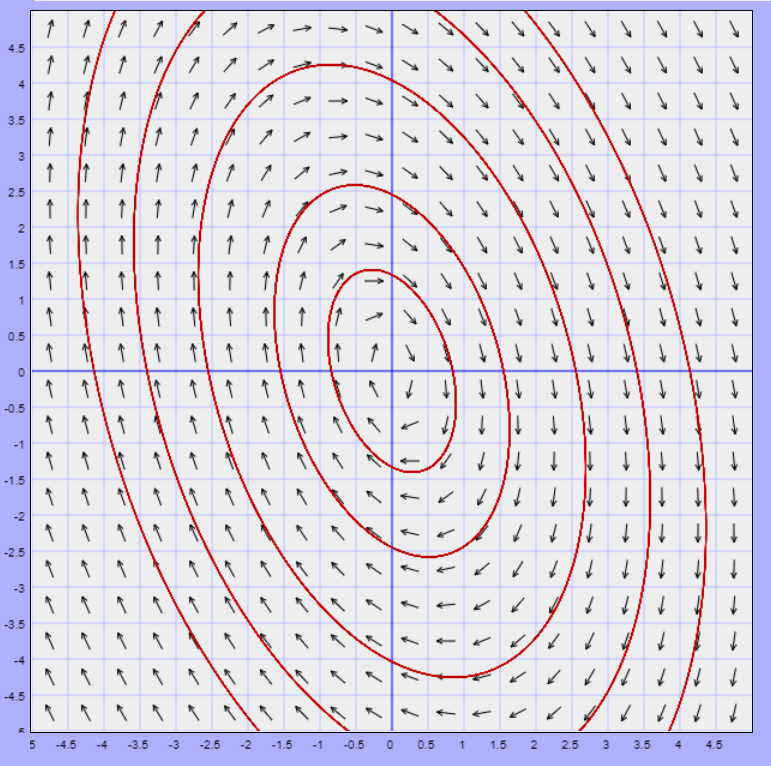
\includegraphics{Images/pplane-a.png}

    \pagebreak

    \item (Click on three solutions in each region)
    \[x' = \begin{bmatrix}
        1 & 1\\
        4 & -2
    \end{bmatrix}x\]
        
    Solution:

    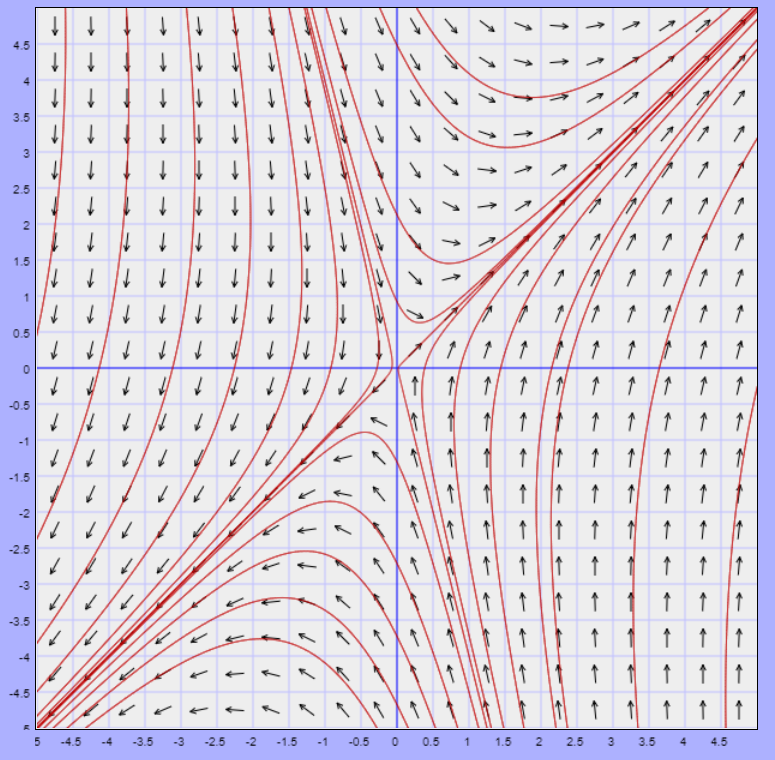
\includegraphics{Images/pplane-b.png}

\end{enumerate}

\pagebreak

\textbf{Use the dsolve command in Python to solve the following systems}
\begin{enumerate}
    \item \[x' = \begin{bmatrix}
        5 & -1\\
        3 & 1
    \end{bmatrix}x\]

    Solution:

    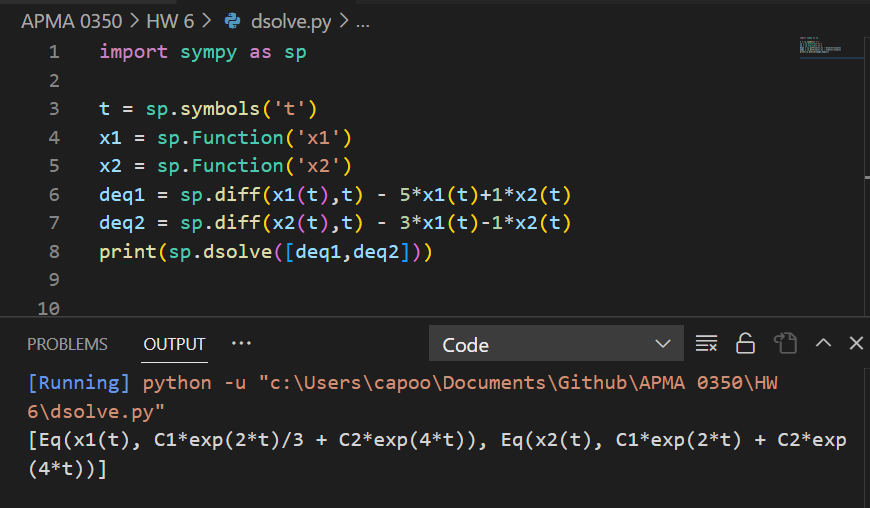
\includegraphics{Images/dsolve-a.png}

    \pagebreak

    \item \[x' = \begin{bmatrix}
        1 & -4\\
        4 & -7
    \end{bmatrix}, \quad x(0) = \begin{bmatrix}
        3\\2
    \end{bmatrix}\]

    Solution:

    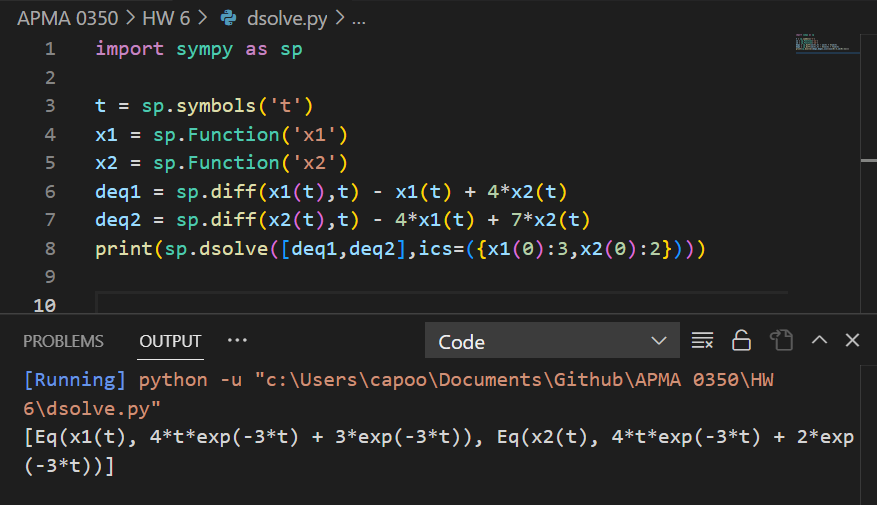
\includegraphics{Images/dsolve-b.png}
\end{enumerate}
\end{document}